\documentclass[main.tex]{subfiles}
\begin{document}

Models of Stochastic Quantum Walks, as introduced above, on different kind of
graphs have been used in the literature to model the remarkably efficient
energy transport phenomena in light-harvesting complexes \cite{Caruso2009}, in
which the external noisy environment plays a fundamental role
\cite{Caruso2014}. Here, we will show how to run a Stochastic Quantum Walk on a
particular kind of graph, the perfect maze, by using the \texttt{QWAK} package.


A perfect maze is defined to be a maze with one and only one path connecting
the entrance with the exit. For example, one can observe, in the random maze in
Fig\ref{fig:mazewalker} that there is only one path connecting the maze
entrance (blue node) to the exit (red node). We can generate a random perfect
maze, by looking at earlier works in the literature \cite{Pozza2022,Caruso2016}
that worked with quantum walks on mazes and then just extract their adjacency
matrix in order to define our Stochastic Quantum Walker on  \texttt{QWAK}. To
properly define the walker we need to specify some additional parameters with
respect to the CTQW case. First, the noise parameter $p \in [0,1]$, that
specifies the amount of noise that our SQW has. If a sink node (or exit node)
is present we also need to specify its index $n$ and the sink rate $\Gamma$ of
the corresponding Linblad operator. We can thus simply instantiate our SQW
object as follows:

\begin{lstlisting}[style=code,escapeinside={__}]
p = 0.1
n = 99
Gamma = 0.99

graph = nx.from_\textunderscore_numpy_\textunderscore_array(maze_\textunderscore_graph.adjacency)
qwak = StochasticQWAK(graph,noiseParam=p,
                      sinkNode=n,sinkRate=Gamma)
\end{lstlisting}

\begin{figure}[!h]
    \centering
    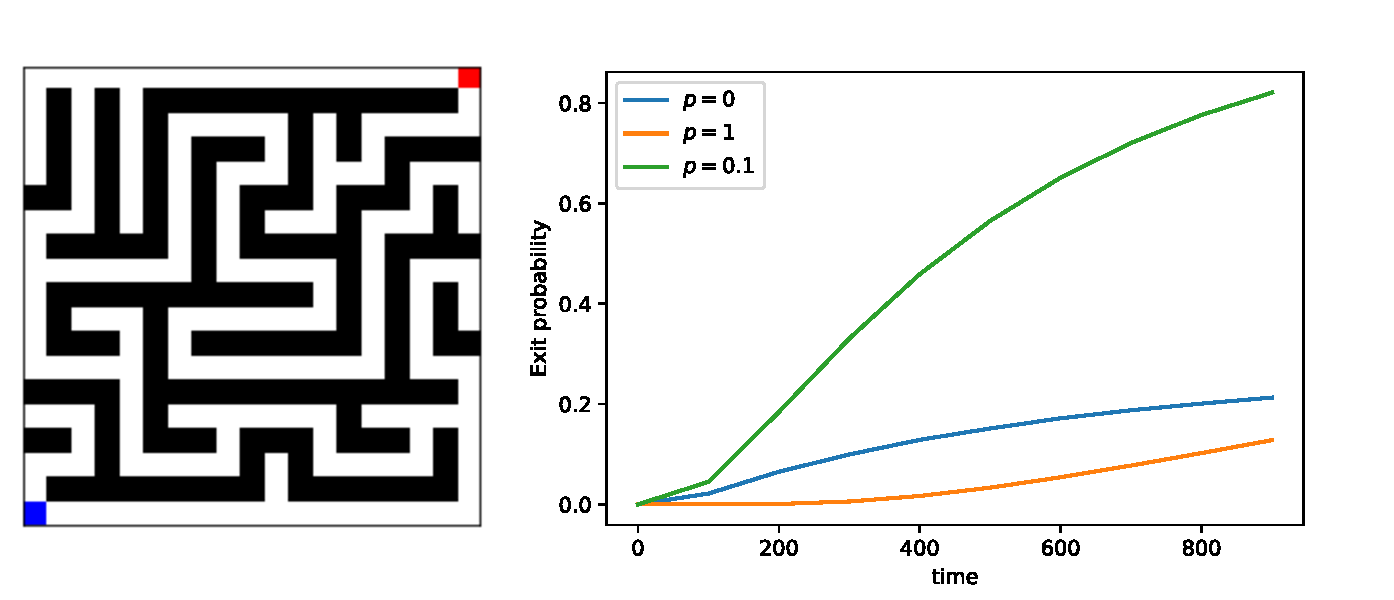
\includegraphics[width=\linewidth]{img/mazewalker.pdf}
    \caption{(Left) A random perfect maze. The walker starts localized on the entrance node (blue) and exits to a sink attached to the exit node (red). (Right) The exit probability of the walker from the sink as a function of time for different values of noise $p$.}
    \label{fig:mazewalker}
\end{figure}

Now that we have instantiated our \texttt{StochasticQWAK} object we can make it
evolve by the usual \texttt{runWalk} command. For example, we can see that if
we run SQWs with different noise parameters $p$ and plot the exit probability
from the sink node as a function of time as reported in
Fig.\ref{fig:mazewalker}, we obtain that the $p=0.1$ walker has a much higher
exit rate than both the purely quantum and purely classical walker ($p=0$ and
$p=1$ respectively). This is a result analogous to well-known noise-assisted
transport phenomena on networks \cite{Caruso2009, mohseni08} that we were able
to reproduce in just a few lines of code with the  \texttt{QWAK} package.


\end{document}
